\chapter{Model sterowania ruchem drogowym}
\label{chap:model}
TODO - tutaj opis ogólny modelu sterowania - sterowanie dyskretne, jakie czujniki co dają, co robi sygnalizator

\section{Opis modelu sterowania}
\label{sec:model_opis}

\begin{figure}[h]
    \centering
    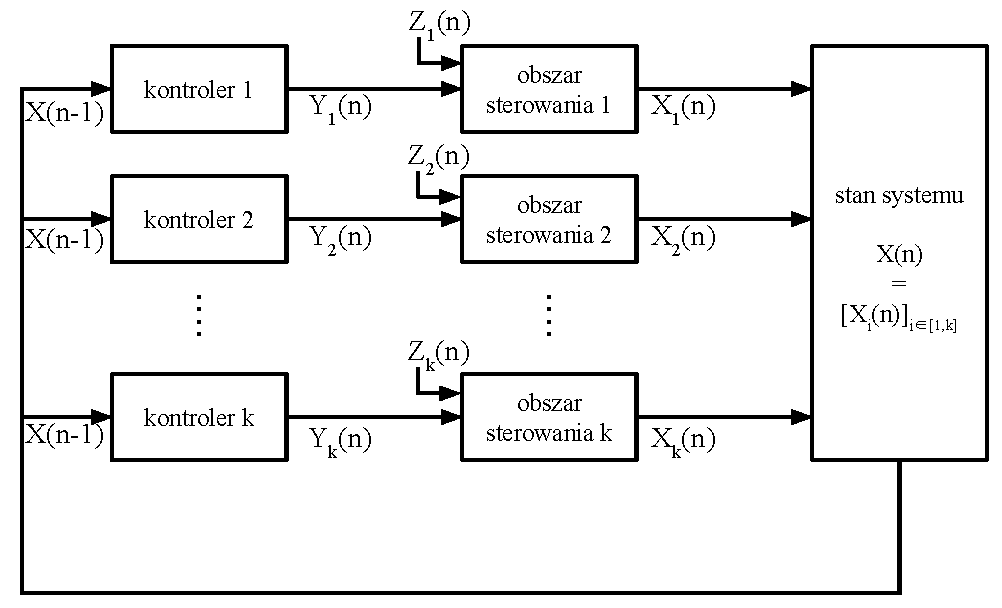
\includegraphics[width=0.8\textwidth]{images/model.pdf}
    \caption{Model systemu sterowania}
    \label{fig:model}
\end{figure}

TODO model jak w \cite{kawalec+sobieszuk-durka} - rys 6 c - czy w rysunku Y i U nie są zamienione?

Na rysunku \ref{fig:model} zaprezentowany został model sterowania ruchem drogowym.
Zespół skrzyżowań objęty sterowaniem podzielony jest na obszary.
Każdy obszar obejmuje pojedyncze skrzyżowanie lub jego autonomiczną część.
Autonomiczną, nazywamy część skrzyżowania, w której dojazd potoków ruchu do miejsca przecięcia nie jest kontrolowany
przez sygnalizatory nie znajdujące się w danej części skrzyżowania.

Każdy obszar sterowany jest przez pojedynczy kontroler.
Kontroler jako dane wejściowe przyjmuje stan systemu w poprzedniej chwili czasu,
który zawiera wielkości mierzone przez czujniki jak i sterowania wyznaczone przez wszystkie kontrolery.

TODO - wszystkie rzeczy z google drive

TODO - co to są zakłócenia i jak wpływają na obiekt sterowany

TODO - struktura sieciowa kontrolerów -kontrolery połączone przez sieć ethernet itp
\cite{kawalec+sobieszuk-durka} rys 7 b - bez centralnego
może opis dlaczego ten a nie rys 7 a
kontroler przekazuje przez stan systemu informacje o swoich sterowaniach

\section{Ograniczenia sterowania ruchem drogowym}
\label{sec:model_ograniczenia}
TODO - ograniczenia sterowania -ograniczenie czasowe, czasy międzyzielone itp